% Options for packages loaded elsewhere
% Options for packages loaded elsewhere
\PassOptionsToPackage{unicode}{hyperref}
\PassOptionsToPackage{hyphens}{url}
%
\documentclass[
  ignorenonframetext,
]{beamer}
\newif\ifbibliography
\usepackage{pgfpages}
\setbeamertemplate{caption}[numbered]
\setbeamertemplate{caption label separator}{: }
\setbeamercolor{caption name}{fg=normal text.fg}
\beamertemplatenavigationsymbolsempty
% remove section numbering
\setbeamertemplate{part page}{
  \centering
  \begin{beamercolorbox}[sep=16pt,center]{part title}
    \usebeamerfont{part title}\insertpart\par
  \end{beamercolorbox}
}
\setbeamertemplate{section page}{
  \centering
  \begin{beamercolorbox}[sep=12pt,center]{section title}
    \usebeamerfont{section title}\insertsection\par
  \end{beamercolorbox}
}
\setbeamertemplate{subsection page}{
  \centering
  \begin{beamercolorbox}[sep=8pt,center]{subsection title}
    \usebeamerfont{subsection title}\insertsubsection\par
  \end{beamercolorbox}
}
% Prevent slide breaks in the middle of a paragraph
\widowpenalties 1 10000
\raggedbottom
\AtBeginPart{
  \frame{\partpage}
}
\AtBeginSection{
  \ifbibliography
  \else
    \frame{\sectionpage}
  \fi
}
\AtBeginSubsection{
  \frame{\subsectionpage}
}
\usepackage{iftex}
\ifPDFTeX
  \usepackage[T1]{fontenc}
  \usepackage[utf8]{inputenc}
  \usepackage{textcomp} % provide euro and other symbols
\else % if luatex or xetex
  \usepackage{unicode-math} % this also loads fontspec
  \defaultfontfeatures{Scale=MatchLowercase}
  \defaultfontfeatures[\rmfamily]{Ligatures=TeX,Scale=1}
\fi
\usepackage{lmodern}

\usetheme[]{metropolis}
\ifPDFTeX\else
  % xetex/luatex font selection
\fi
% Use upquote if available, for straight quotes in verbatim environments
\IfFileExists{upquote.sty}{\usepackage{upquote}}{}
\IfFileExists{microtype.sty}{% use microtype if available
  \usepackage[]{microtype}
  \UseMicrotypeSet[protrusion]{basicmath} % disable protrusion for tt fonts
}{}
\makeatletter
\@ifundefined{KOMAClassName}{% if non-KOMA class
  \IfFileExists{parskip.sty}{%
    \usepackage{parskip}
  }{% else
    \setlength{\parindent}{0pt}
    \setlength{\parskip}{6pt plus 2pt minus 1pt}}
}{% if KOMA class
  \KOMAoptions{parskip=half}}
\makeatother


\usepackage{longtable,booktabs,array}
\usepackage{calc} % for calculating minipage widths
\usepackage{caption}
% Make caption package work with longtable
\makeatletter
\def\fnum@table{\tablename~\thetable}
\makeatother
\usepackage{graphicx}
\makeatletter
\newsavebox\pandoc@box
\newcommand*\pandocbounded[1]{% scales image to fit in text height/width
  \sbox\pandoc@box{#1}%
  \Gscale@div\@tempa{\textheight}{\dimexpr\ht\pandoc@box+\dp\pandoc@box\relax}%
  \Gscale@div\@tempb{\linewidth}{\wd\pandoc@box}%
  \ifdim\@tempb\p@<\@tempa\p@\let\@tempa\@tempb\fi% select the smaller of both
  \ifdim\@tempa\p@<\p@\scalebox{\@tempa}{\usebox\pandoc@box}%
  \else\usebox{\pandoc@box}%
  \fi%
}
% Set default figure placement to htbp
\def\fps@figure{htbp}
\makeatother

\ifLuaTeX
  \usepackage{luacolor}
  \usepackage[soul]{lua-ul}
\else
  \usepackage{soul}
  \makeatletter
  \let\HL\hl
  \renewcommand\hl{% fix for beamer highlighting
    \let\set@color\beamerorig@set@color
    \let\reset@color\beamerorig@reset@color
    \HL}
  \makeatother
\fi




\setlength{\emergencystretch}{3em} % prevent overfull lines

\providecommand{\tightlist}{%
  \setlength{\itemsep}{0pt}\setlength{\parskip}{0pt}}



 


\setbeamerfont{title}{size=\large}
\makeatletter
\@ifpackageloaded{caption}{}{\usepackage{caption}}
\AtBeginDocument{%
\ifdefined\contentsname
  \renewcommand*\contentsname{Table of contents}
\else
  \newcommand\contentsname{Table of contents}
\fi
\ifdefined\listfigurename
  \renewcommand*\listfigurename{List of Figures}
\else
  \newcommand\listfigurename{List of Figures}
\fi
\ifdefined\listtablename
  \renewcommand*\listtablename{List of Tables}
\else
  \newcommand\listtablename{List of Tables}
\fi
\ifdefined\figurename
  \renewcommand*\figurename{Figure}
\else
  \newcommand\figurename{Figure}
\fi
\ifdefined\tablename
  \renewcommand*\tablename{Table}
\else
  \newcommand\tablename{Table}
\fi
}
\@ifpackageloaded{float}{}{\usepackage{float}}
\floatstyle{ruled}
\@ifundefined{c@chapter}{\newfloat{codelisting}{h}{lop}}{\newfloat{codelisting}{h}{lop}[chapter]}
\floatname{codelisting}{Listing}
\newcommand*\listoflistings{\listof{codelisting}{List of Listings}}
\makeatother
\makeatletter
\makeatother
\makeatletter
\@ifpackageloaded{caption}{}{\usepackage{caption}}
\@ifpackageloaded{subcaption}{}{\usepackage{subcaption}}
\makeatother

\usepackage{bookmark}
\IfFileExists{xurl.sty}{\usepackage{xurl}}{} % add URL line breaks if available
\urlstyle{same}
\hypersetup{
  pdfauthor={Giorgio Arcara},
  hidelinks,
  pdfcreator={LaTeX via pandoc}}


\author{Giorgio Arcara}
\date{}

\begin{document}


\begin{frame}
% TITLE SLIDES
\title{Metodi Statistici per la Neuropsicologia Forense}
\author{Giorgio Arcara,\\ Università di Padova \\ IRCCS San Camillo, Venezia}

\titlegraphic{

 \vspace*{7cm}

\includegraphics[scale=0.15]{Figures/LogoSanCamilloIRCCS_Unipd_alpha.png}
\hfill 
\includegraphics[scale=0.15]{Figures/CC_license_3_0.png}
}
\date{\today}
\maketitle
\end{frame}

\begin{frame}{Lezione di oggi}
\phantomsection\label{lezione-di-oggi}
\begin{itemize}[<+->]
\tightlist
\item
  Presentazione del docente e del corso.
\item
  Aspetti organizzativi del corso.
\item
  Obiettivi formativi.
\end{itemize}
\end{frame}

\section{Introduzione}\label{introduzione}

\begin{frame}{CV Giorgio Arcara}
\phantomsection\label{cv-giorgio-arcara}
\footnotesize

\begin{itemize}[<+->]
\item
  Laurea in Psicologia presso Unipd 2005)
\item
  Master in Neuropsicologia dei disturbi cognitivi acquisiti (2006)
\item
  vari post-doc presso dipartimenti di psicologia, neuroscienze,
  ingegneria
\item
  Dal 2016 Ricercatore presso IRCCS San Camillo di Venezia.
\item
  Dal 2025 Professore Associato in Psicometria - Università di Padova.
\end{itemize}

\pause

\hfill
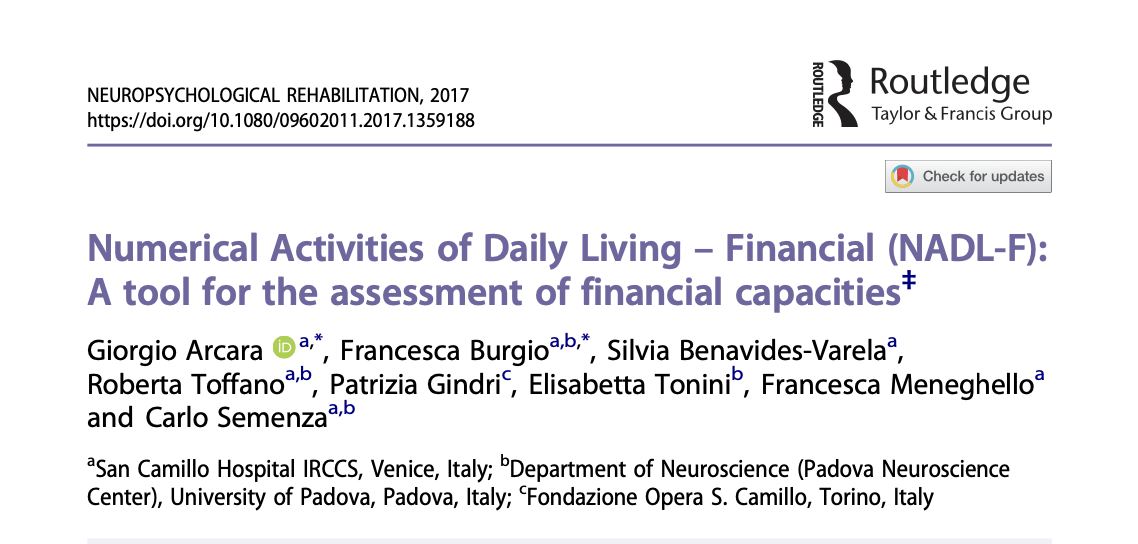
\includegraphics[width=0.6\linewidth,height=\textheight,keepaspectratio]{Figures/NADL_F.png}
\end{frame}

\begin{frame}{Contatti e riferimenti}
\phantomsection\label{contatti-e-riferimenti}
\centering

\href{https://giorgioarcara.github.io}{\ul{https://giorgioarcara.github.io}}

\href{https://www.dpg.unipd.it/category/ruoli/personale-docente?key=4D0707A2DD6FCCD50B90E4C9F316A625}{\ul{pagina
personale unipd}}

\href{mailto:giorgio.arcara@unipd.it}{\nolinkurl{giorgio.arcara@unipd.it}}
\end{frame}

\begin{frame}{Aspetti organizzativi - Lezioni}
\phantomsection\label{aspetti-organizzativi---lezioni}
\begin{itemize}[<+->]
\tightlist
\item
  Lezioni online principalmente il giovedì e il venerdì (dalle 11.30
  alle 13.00 circa)
\item
  Le lezioni prevedono didattica frontale (interattiva), esercitazioni
  in classe.
\item
  Saranno trattate poche formule, molto approfonditamente.
\item
  Sono benvenute le domande (in qualsiasi momento).
\item
  Sarà utilizzato il software R, che è raccomandato. Saranno forniti
  script di R e sarà spiegato come utilizzarli, ma non è necessario
  conoscere R per il corso.
\end{itemize}
\end{frame}

\begin{frame}{Aspetti organizzativi - Materiali}
\phantomsection\label{aspetti-organizzativi---materiali}
\textbf{Condividerò tutto il materiale utilizzato e mostrato}

I materiali principali sono le slides e materiali aggiuntivi che vi
saranno forniti durante il corso. I materiali li troverete anche al
link:

\href{\%5Bhttps://github.com/giorgioarcara/stat_forensic_neuropsy}{\ul{https://github.com/giorgioarcara/stat\_forensic\_neuropsy}}

Condividerò anche script di R e sarà dato risalto a ``simulazioni'' di
dati per comprensione dei concetti, con script sviluppati durante il
corso.
\end{frame}

\begin{frame}{Aspetti organizzativi - Materiali}
\phantomsection\label{aspetti-organizzativi---materiali-1}
\begin{columns}
\column{0.5\textwidth}

\emph{Mondini, S., Cappelletti, M., \& Arcara, G. (2022). Methodology in Neuropsychological Assessment: An Interpretative Approach to Guide Clinical Practice. Taylor \& Francis.}

\column{0.5\textwidth}

\begin{figure}

\includegraphics[scale=0.5]{Figures/Methodology_book.png}
\end{figure}

\end{columns}
\end{frame}

\begin{frame}{Aspetti organizzativi - Materiali aggiuntivi}
\phantomsection\label{aspetti-organizzativi---materiali-aggiuntivi}
\begin{itemize}[<+->]
\item
  Libro gratuito su statistica base ed R
  \{\underline{https://learningstatisticswithr.com/}
\item
  Libro gratuito su psicometria (più avanzato)
  \underline{https://personality-project.org/r/book/}
\end{itemize}
\end{frame}

\begin{frame}{Aspetti organizzativi - Esami}
\phantomsection\label{aspetti-organizzativi---esami}
Gli esami saranno scritti con:

\begin{itemize}[<+->]
\tightlist
\item
  domande aperte su aspetti teorici.
\item
  domande su scenari applicativi in cui ragionare per applicare le
  conoscenze sviluppate.
\end{itemize}

Gli esami saranno poco nozionistici e più di ragionamento

\underline{Non sarà necessario ricordare a memoria nessuna formula}
\end{frame}

\begin{frame}{Obiettivi del corso}
\phantomsection\label{obiettivi-del-corso}
Partiamo dalla fine:

\begin{itemize}[<+->]
\tightlist
\item
  Fornire elementi di conoscenza statistica e ragionamento critico utili
  per la neuropsicologia forense
\item
  Fornire conoscenze sia per la pratica di psicologia forense, sia per
  chi vuole fare ricerca in ambito forense.
\item
  Fornire conoscenze sull'elemento cardine per la valutazione forense:
  il test cognitivo o neuropsicologico, con le sue potenzialità e
  limiti.
\end{itemize}

\emph{Obiettivo bonus}: superare alcuni traumi che vi ha dato la
statistica a Psicologia
\end{frame}

\begin{frame}{Perché è utile la statistica per il neuropsicologo
forense?}
\phantomsection\label{perchuxe9-uxe8-utile-la-statistica-per-il-neuropsicologo-forense}
\begin{columns}
\column{0.5\textwidth}

\begin{figure}
\includegraphics[width=0.8\textwidth]{Figures/Motore.png}
\end{figure}
\tiny{Non serve conoscere come funziona un motore per guidare una macchina. Basta sapere cosa è giusto o sbagliato fare con pedali, cambio e volante. (Aforisma approssimativo di H. R. Baayen, 2008 circa)}


\column{0.5\textwidth}

\begin{figure}
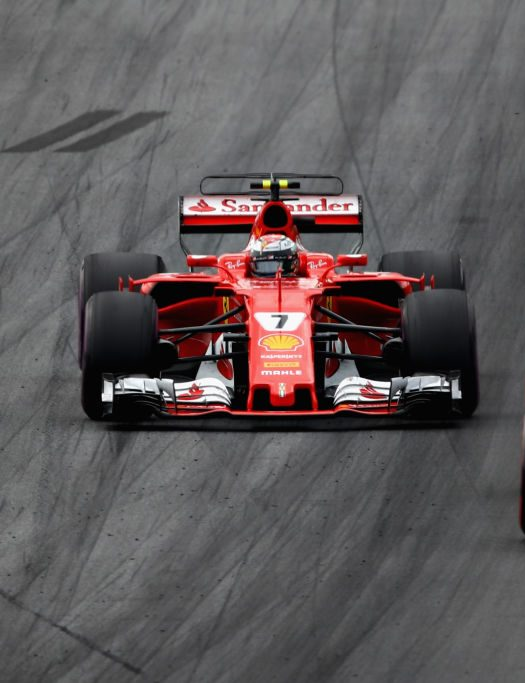
\includegraphics[width=0.8\textwidth]{Figures/F1.png}
\end{figure}
\tiny{I piloti di formula 1 hanno conoscenze superiori su come funziona un motore.}

\end{columns}
\end{frame}

\begin{frame}{5 principi basilari di questo corso (1)}
\phantomsection\label{principi-basilari-di-questo-corso-1}
\begin{enumerate}[<+->]
\tightlist
\item
  la valutazione neuropsicologica forense è innanzitutto una valutazione
  clinica
\end{enumerate}

\vspace{3em}

\emph{Per una buona perizia, bisogna avere competenze cliniche (in
particolare sono rilevanti le capacità diagnostiche)}
\end{frame}

\begin{frame}{5 principi basilari di questo corso (2)}
\phantomsection\label{principi-basilari-di-questo-corso-2}
\begin{enumerate}[<+->]
\setcounter{enumi}{1}
\tightlist
\item
  In questo corso di Laurea (non solo nelle mie lezioni) il leitmotiv
  sarà che la valutazione forense hanno un ruolo fondamentale
  valutazioni di tipo cognitivo.
\end{enumerate}

\vspace{3em}

\emph{Un approccio che si sta imponendo in ambito forense è quello Di
sostanziare in maniera il più obiettiva/oggettiva possibile le vostre
argomentazioni.}

\emph{Questo si contrappone ad un approccio dominante alla valutazione
forense come semplice giudizio clinico, magari da fonte autorevole, o i
test proiettivi, etc.)}
\end{frame}

\begin{frame}{Valutazione qualitativa}
\phantomsection\label{valutazione-qualitativa}
\begin{center}
\begin{tikzpicture}[baseline=(current bounding box.center)]

% Prima riga: sbagliato - giusto
\node[anchor=west] at (0, 0) {\textbf{Sbagliato}};
\node[anchor=east] at (10, 0) {\textbf{Giusto}};
\draw[thick] (1.8, 0) -- (8.5, 0);

% X al centro
\node[text=red, font=\bfseries\Huge] at (5, 0) {X};

% Seconda riga: peggio - meglio
\node[anchor=west] at (0, -1.2) {\textbf{Peggio}};
\node[anchor=east] at (10, -1.2) {\textbf{Meglio}};
\draw[thick] (1.5, -1.2) -- (8.5, -1.2);

\end{tikzpicture}
\end{center}
\end{frame}




\end{document}
